\section{WORKBOOK LESSON 4
RAJA YOGA}
 

Raja Yoga is the most powerful influence in the chart. It literally means an astrological combination (yoga) that creates a king (raja), but indicates power, affluence and authority of all types. There are many different types and levels of Raja Yoga. There is hardly a chart without some sort of Raja Yoga, either from the Lagna or the Moon. Such Yogas may not bring extraordinary results however. Yet even in a weak chart they will give improved fortune during their periods and subperiods.

 

Raja Yogas are caused by single planets, like Saturn for Libra Ascendant, or combinations of planets, like Mercury and the Moon, the ninth and the tenth lords for Libra. Combination Raja Yogas are stronger. Combination Raja Yogas are yet stronger if they include single Raja Yoga planets.

 
\begin{enumerate}
\item Raja Yoga is produced by any combination of trine lords (1, 5, 9) and angle lords (1, 4, 7, 10).
\item The ninth is the best trine followed by the fifth and the first. The tenth is the best angle followed by the fourth, the first and the seventh.
\end{enumerate}
 

Raja Yogas therefore involving the seventh lord are rather weak and not counted by all Vedic astrologers. We would advise beginning students not to consider such Raja Yoga combinations unless they are included among other stronger combinations. Raja Yogas involving the first lord are not strong. However, if the first lord is involved with a Raja Yoga planet, like Venus and Saturn for Libra, or a combination of Raja Yoga planets, like Mars with the Sun and Moon for Aries, then the Yoga becomes stronger. With the inclusion of the first lord it impacts the native more on a personal level.

 

Besides house rulership Raja Yogas are enhanced if the planets involved are in their own signs or exalted, are friendly to one another naturally or temporally, or occur relative to the Moon as well as the Lagna. Yet Raja Yogas in Duhsthanas (6, 8, 12) can be effective, like the case of a politician who goes from prison to power.

 

A powerful Raja Yoga, like between the ninth and tenth lords, can neutralize all other difficulties in the chart. On the other hand, a weak chart, in which the Ascendant and its lord are highly afflicted cannot even be saved by a Raja Yoga.

 

Raja Yoga gives the ability to fulfill ones Dharma in life. Such Yogas commonly bestow power, fame or wealth. It is relative to the nature of the chart as to whether they are part of a spiritual, intellectual, business, or political life or several of these domains at the same time They always give a person prominence in life, whatever field they are in. They serve to strengthen other Yogas in the chart including Dhana Yogas (combinations for wealth) and combinations for knowledge or creativity.

 

Relative to the spiritual life Sannyasa Yogas, combinations for renunciation, may be better than Raja Yogas. However Raja Yogas involving the fifth and ninth lords usually give spiritual rewards as well, particularly if they involved Sattvic planets (Sun, Moon, and Jupiter), or are reinforced by other spiritual combinations in the chart.

 



\subsection{Raja Yoga Planets and Divisional Charts}

 

The details of divisional charts are basically beyond the scope of this introductory course. However we do want to introduce some principles for them. The first is that the same basic principles applied to the birthchart are useful in divisional charts as well, including the existence of Raja Yogas. There are a few Vedic astrologers who do not read aspects from the divisional charts but only positions. However most do read aspects as well.

 

Raja Yoga is the most significant of all Yogas and helps introduce the student into this line of thought. In the following example, we will show how it applies both in the birthchart and in divisional charts.

 

\subsection{Raja Yoga Example Chart}

I have chosen the chart of  Deepak Chopra, who has been an extraordinarily successful writer, doctor, and television personality in the field of natural healing. Clearly one would expect some Raja Yogas in the chart for such recognition to occur.

 

\paragraph{The Birthchart}

 


 \begin{figure}[h]
\centering
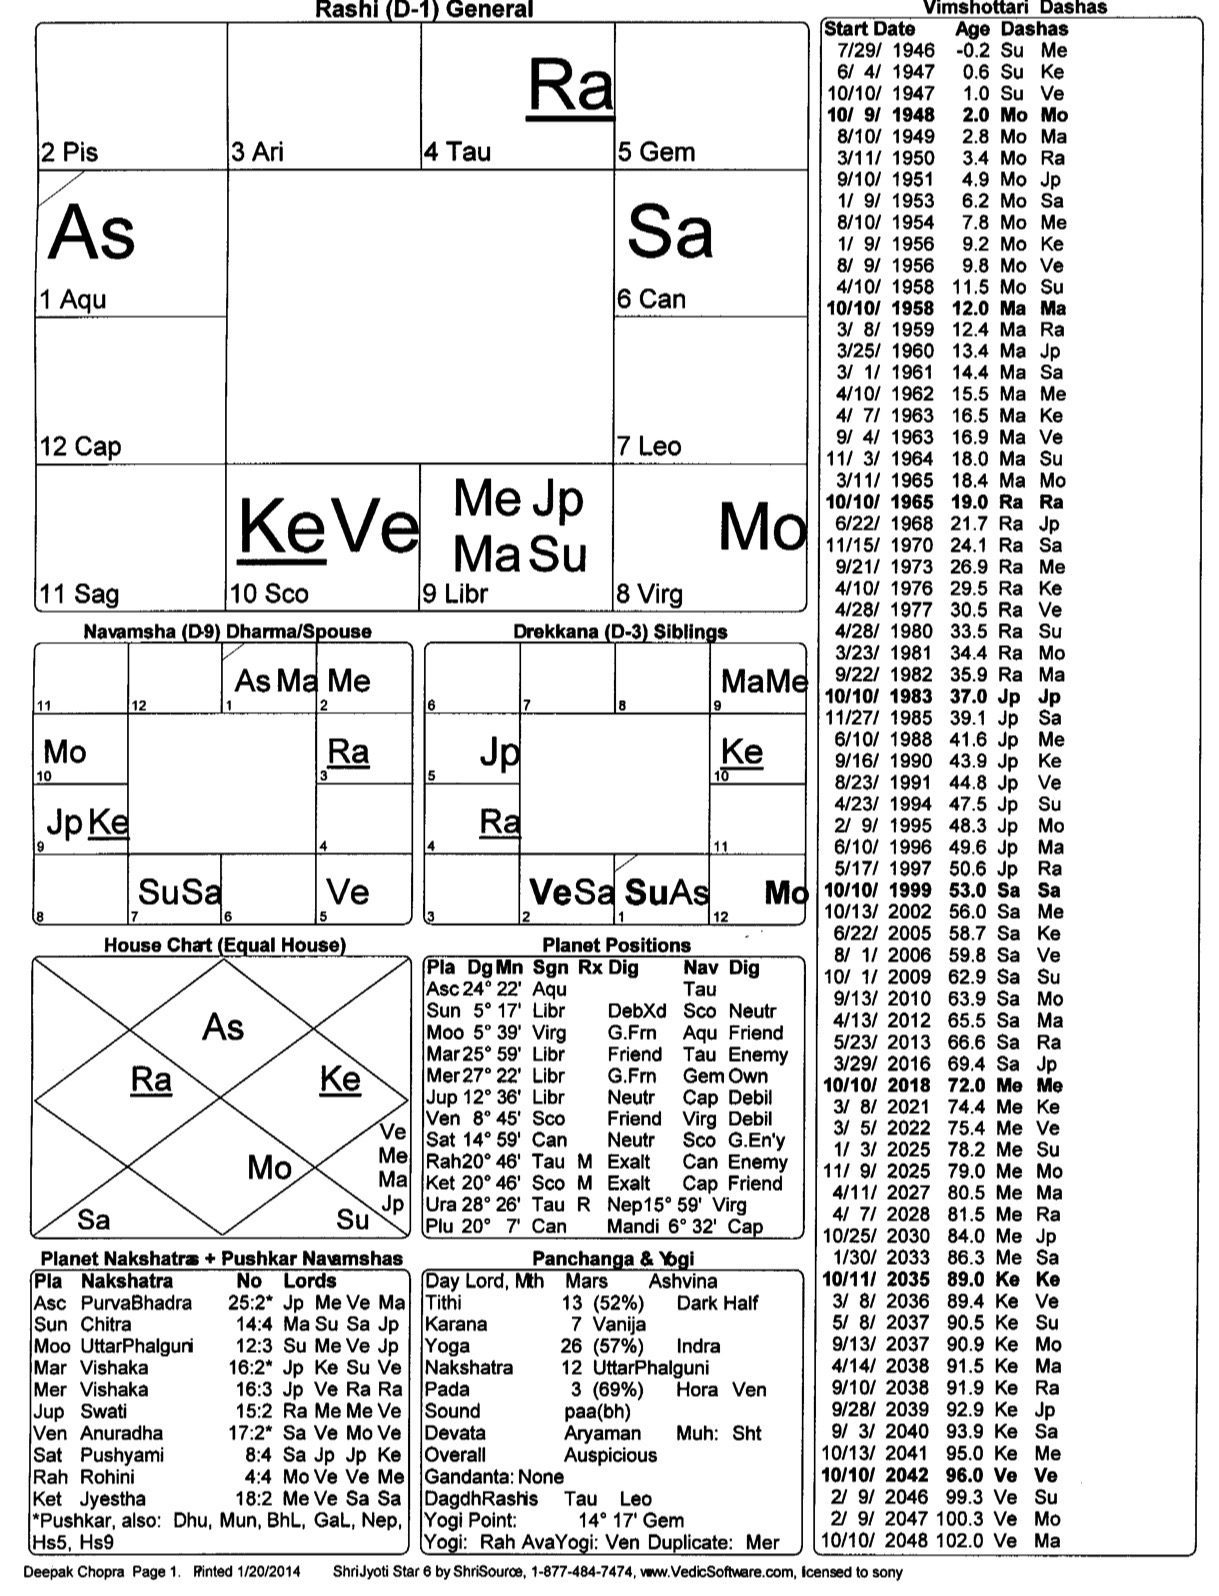
\includegraphics[width=10cm]{pics/Deepak-Chopra1.jpg}
\caption{}
\end{figure}
 

 \begin{figure}[h]
\centering
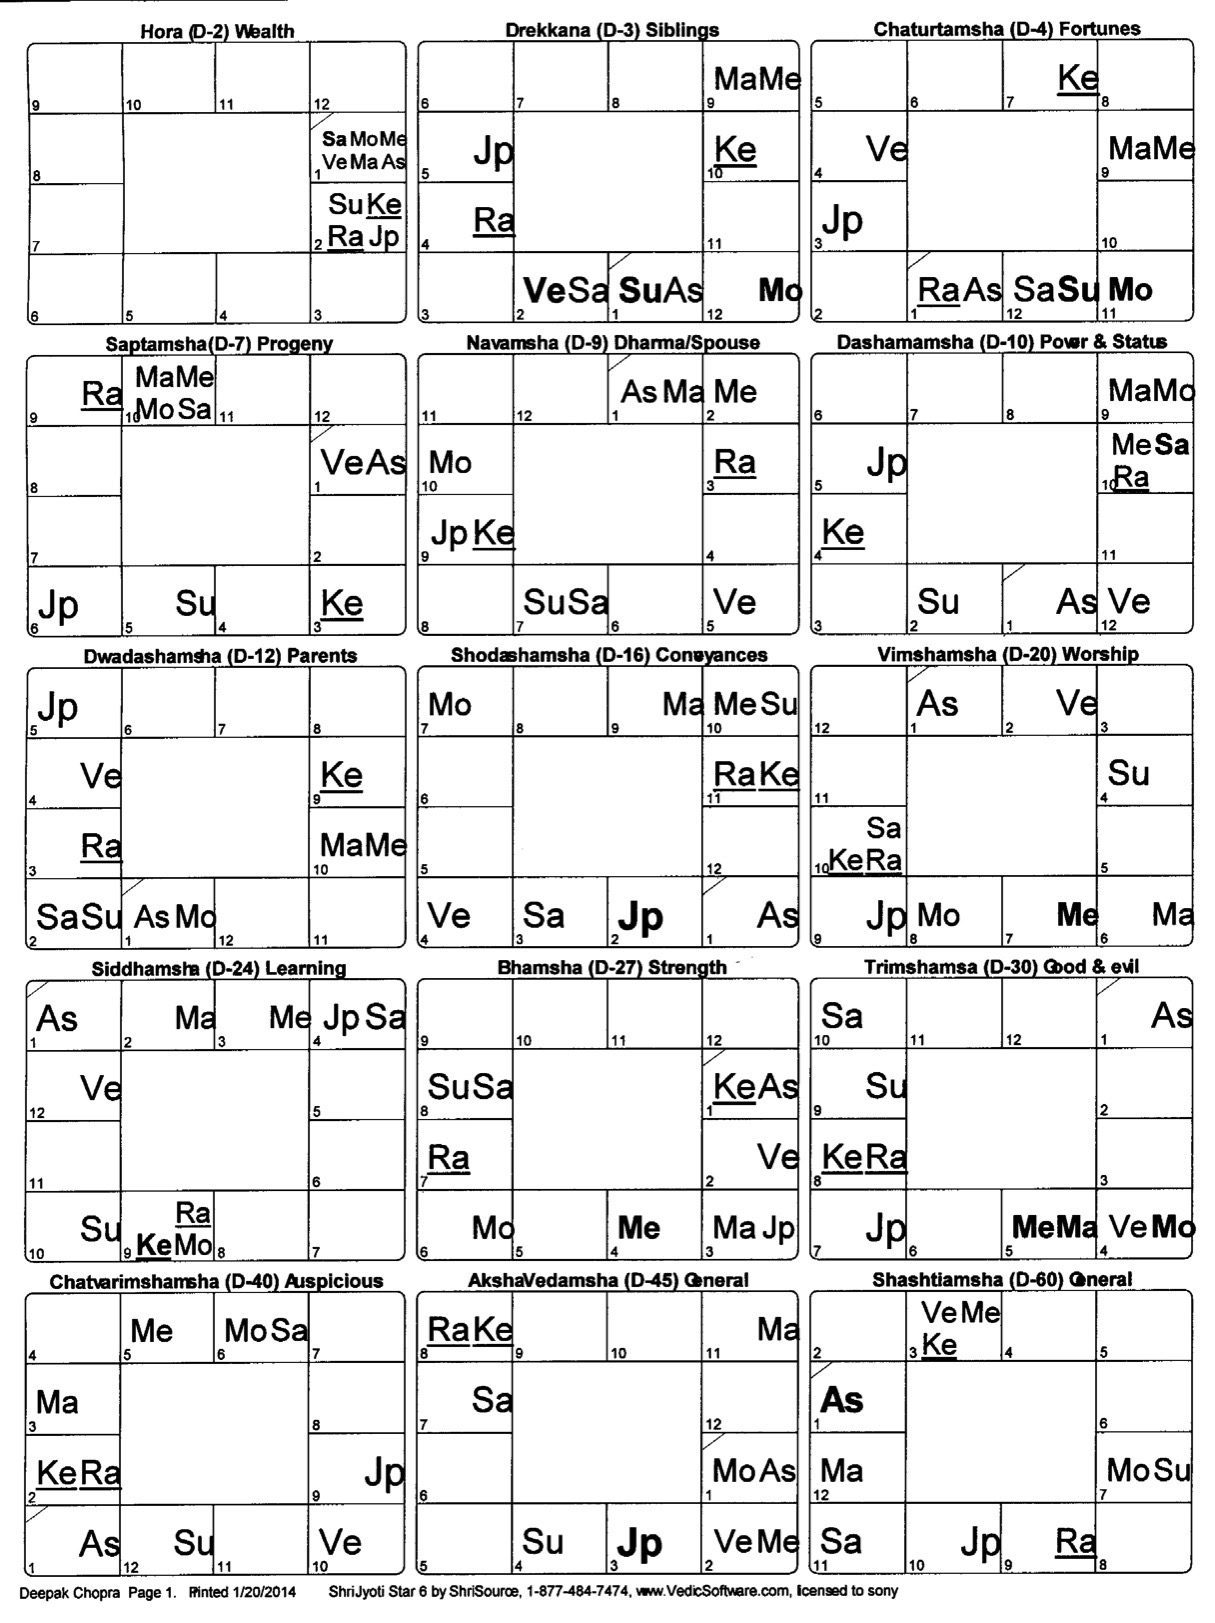
\includegraphics[width=10cm]{pics/Deepak-Chopra2.jpg}
\caption{}
\end{figure}

 

\paragraph{From the Ascendant}

 

The birthchart is dominated by the strongest of all Raja Yogas, an exchange of houses between the ninth and tenth lords. Here Venus the lord of the ninth is located in Scorpio, a sign of Mars, in the tenth house, while Mars, the lord of the tenth, is in Libra, a sign of Venus, the ninth house. Rahu, in a sign of Venus in the fourth and Ketu in a sign of Mars in the tenth are strengthened by this Yoga and give it yet more power. Rahu is in an angle, the fourth house, aspected by Venus, ruler of a trine, the ninth, which is another type of Raja Yoga. This mutual exchange is also the final dispositor of all the other planets in the chart. Such a Venus-Mars Raja Yoga gives great charisma.

In addition Mercury, the fifth lord, is with Mars, the tenth lord, in the ninth house, creating another Raja Yoga, this time involving the intellect and creative intelligence (the fifth house). As Mercury is also the fifth lord of children, the son of the native has himself gained success as a writer. Jupiter combines as the second and eleventh lord giving great income and creating a Dhana Yoga. It also increases powers of speech and writing (second house lordship). Jupiter carries the influence of these planets in the ninth house to the Ascendant by its trine aspect. The Sun, though debilitated, participates in this Raja Yoga through its location in the ninth house, making it auspicious and powerful as well. These four planets in the ninth house, including the tenth lord, constitute a Sannyasa Yoga or combination for renunciation. This strengthens the spiritual influence of the planets involved and gives the person the ability to look beyond his success to transcendent goals in life.

 

Saturn as a malefic does well in the sixth house as the Ascendant lord and is under no adverse aspects. The Moon as the sixth lord in the eighth house and Saturn as the twelfth lord in the sixth house are not bad either because they create a Vipreet or reverse Raja Yoga. This occurs when the lords of Duhsthanas (6, 8 and 12) occupy other Duhsthanas and are otherwise not afflicted. Yet this Yoga is not strong in itself because Moon and Saturn do not exchange signs. All the planets in the chart, therefore, are involved with Raja Yogas to some degree or another.

 

\paragraph{From the Moon}

From the Moon sign, Mercury, the lord of the first, a trine house, is conjoined with Jupiter, lord of the fourth, an angular house, creating another Raja Yoga in the second house from the Moon, the house of speech. The Mars-Venus exchange occurring between the second and third houses from the Moon does not constitute a Raja Yoga here but it does further strengthen the second house from the Moon and the Raja Yoga within it. Saturn is well placed eleventh from the Moon as the fifth lord aspecting its own house, giving gains and abundance. So the Moon chart supports, though does not entirely elevate the Raja Yogas in the birthchart.

 

\paragraph{Navamsha}

The Navamsha is used for all indications in life as a fine tuning mechanism for the birthchart. Saturn as the lord of the ninth and tenth by itself gives Raja Yoga in the Navamsha. The Sun as the fourth lord, a malefic ruling an angle, contributes to this. Mars does not harm this Raja Yoga because Mars is the tenth lord in the birthchart.

 

Another interesting position occurs there. Mercury as Atma Karaka (the planet with the highest number of degrees and minutes in any sign) is the final dispositor in the Navamsha from the second house of speech and writing. While this is not a Raja Yoga, it does strengthen Mercury and the second house, with its writing and speaking potentials.

 

One notices that both Venus and Jupiter are debilitated in the Navamsha. However both are located in auspicious trine houses, so that their debility does not cause much problem. Venus as Lagna lord in the fifth is a good position, as is Jupiter as eleventh lord in the ninth. The Moon in the tenth house is another good position.

 

\paragraph{Drekkana}

The Drekkana not only indicates brothers and sisters but our own vital energy, curiosity and interests. It shows the expression of our Prana or life-force. As such it is relevant not only to health but to all creative endeavors and to career as well. In fact I use the Drekkana like the Rashi and Navamsha to examine all affairs in life. It fine-tunes the positions in the birthchart. For example, a person with the Gemini Drekkana of Libra rising will have intellectual Gemini traits.

 

In this instance the Drekkana Lagna is Libra. Venus, the lord of Lagna, combines with Saturn, the Yoga Karaka planet, creating another strong Raja Yoga in the second house of speech.

 

Mercury again is final dispositor in the chart from its position in the benefic ninth house in its own sign Gemini. It is combined with the second lord Mars, which is also the tenth and third lord in the birthchart, increasing the indications of each in the third divisional chart. Mercury and Mars are aspected by Jupiter from the fifth house of creative intelligence. Mercury disposes of an otherwise weak Moon in the twelfth house and makes it beneficial. The Moon as the tenth lord in Virgo also shows working in a foreign country. The Sun as eleventh lord in the Ascendant, aspected by Jupiter, gives gains and has its debility cancelled.

 

\paragraph{Dashamsha}

The Dashamsha as the tenth divisional is specifically related to the tenth house of career. First we look at the general strength of the birthchart. As the birthchart has strong career indications we look for their confirmation in the Dashamsha. We do this in two ways, first by noting the general strength of the Dashamsha chart and second by noting the position of the tenth lord within it.

 

The Dashamsha contains several powerful Raja Yogas. Its Ascendant is Libra again. Mercury, lord of the ninth is located in the tenth house in Cancer, the sign of the Moon. The Moon, lord of the tenth, is in the ninth in Gemini, a sign of Mercury. Again this is a mutual exchange of the ninth and tenth sign rulers, the strongest Raja Yoga. In addition Saturn, the Yoga Karaka for Libra, is located along with Mercury in the tenth house making this Yoga yet stronger. The Rahu-Ketu axis in the tenth and fourth houses ruled by the Moon and Saturn contribute to this Raja Yoga. Rahu in an angle along with a trine lord is another Raja Yoga. Both Saturn and Mercury with Rahu are trine lords.

 

Auspicious Jupiter in the fifth aspects the Ascendant and the Moon. The Sun as the eleventh lord in the second gives gains. Venus in the twelfth again can show one working overseas, though it does have some weakness here being debilitated and influenced by Mars and Saturn. Raja Yogas, by their prominence, can give their stress as well, which may be indicated by other weaker planets in the chart.

 

Mars, the tenth lord in the birthchart, is in the ninth house of the Dashamsha along with the tenth lord of Dashamsha. Mercury, the tenth lord from the Moon in the birthchart, is located in the tenth house of the Dashamsha. Its position as Atma Karaka also gives it more strength here as well.

 

As both the Dashamsha chart is strong in itself and the tenth in the birthchart is strong as well, good results can be expected. Had the birthchart been weak in regard to tenth house affairs, the best Dashamsha in the world would not make much difference. If the birthchart were strong in tenth house matters but the Dashamsha weak then the natives career would be generally good but seldom extraordinary.

 

\paragraph{Dashas}

The natives rise to recognition occurred along with Jupiter Dasha that started in Oct. 1983, particularly from Jupiter-Saturn, the subperiod of the Lagna lord, which began in November of 1985. Often the main effects of Dashas dont begin until the subperiod of the Lagna lord is crossed.

 

Taking the Dasha lord, Jupiter in Libra, as the Ascendant is a good way to judge Dasha results. From there Saturn is in the tenth house in Cancer as Yoga Karaka and under no malefic aspects. Saturn aspects the tenth house and the tenth lord giving a powerful rise in career. Mars and Venus exchange as first and second lords giving powers of speech and income.

 

The Jupiter-Mercury period from June of 1988 to September of 1990 was very good for writing as well. Jupiter-Venus and Jupiter-Mars, with subperiods of the ninth and tenth lords would also prove quite extraordinary.

 

The Saturn Dasha commenced in Oct. 1999. In this case Saturn as a malefic is well placed in the sixth house, which as an upachaya house and a late maturing planet would bring continued growth and development. Taking the position of Saturn in the birthchart as the Ascendant the Venus-Mars exchange is of the fourth and fifth lords, another Raja Yoga.

 

However Saturn cannot be as expansive a planet as Jupiter. That is simply not its nature. Yet as the Ascendant Lord is likely to bring out the full potential of the chart. Hence one could expect that the person will enter into a period of consolidation under Saturn. Saturn in an upachaya house, the sixth, is also quite strong. Such consolidation will bring very good results.

 

As Saturn is in the sixth house of the birthchart both enemies and litigation can be expected but with the same indication that the native can overcome them and prosper. Saturns position in the eleventh from the Moon is also a point of income, prominence and a degree of danger. The native may have to orient his work in a way that is more personally fulfilling or more spiritual in nature. Nevertheless it will be a period of continued prominent work and expression with few limitations.

 

\subsection{Raja Yoga Chart 2
Political Raja Yoga}
 

Raja Yoga is of course very important in the charts of politicians and world leaders. Their charts invariably have such combinations. But having such combinations is not enough to make a person President or give them the highest position. A politicians chart has to be very strong even for them to run for high office.

 

The following is the chart of Walter Mondale, Senator, Vice-President and Presidential candidate. I have chosen this chart because it contains a similar Yoga to the previous chart. The Ascendant is Aquarius with a combination of Mars and Venus, the ninth and tenth lords in the tenth house, the same type of Raja Yoga. In this case the Yoga combines with Saturn, the Ascendant lord, which makes it more powerful. The tenth lord is in its own house creating a Mangala Yoga or Maha Purusha Yoga of the planet Mars. The Yoga has the additional strength of Ketu, which serves to carry the influence of the planets with which it is conjoined. Rahu in an angle aspected by Venus, a trine lord, is another mild Raja Yoga. In addition Jupiter aspects the tenth house from its own sign in the second, giving both wealth and power. This is an extraordinary tenth house giving international status and recognition.

 \begin{figure}[h]
\centering
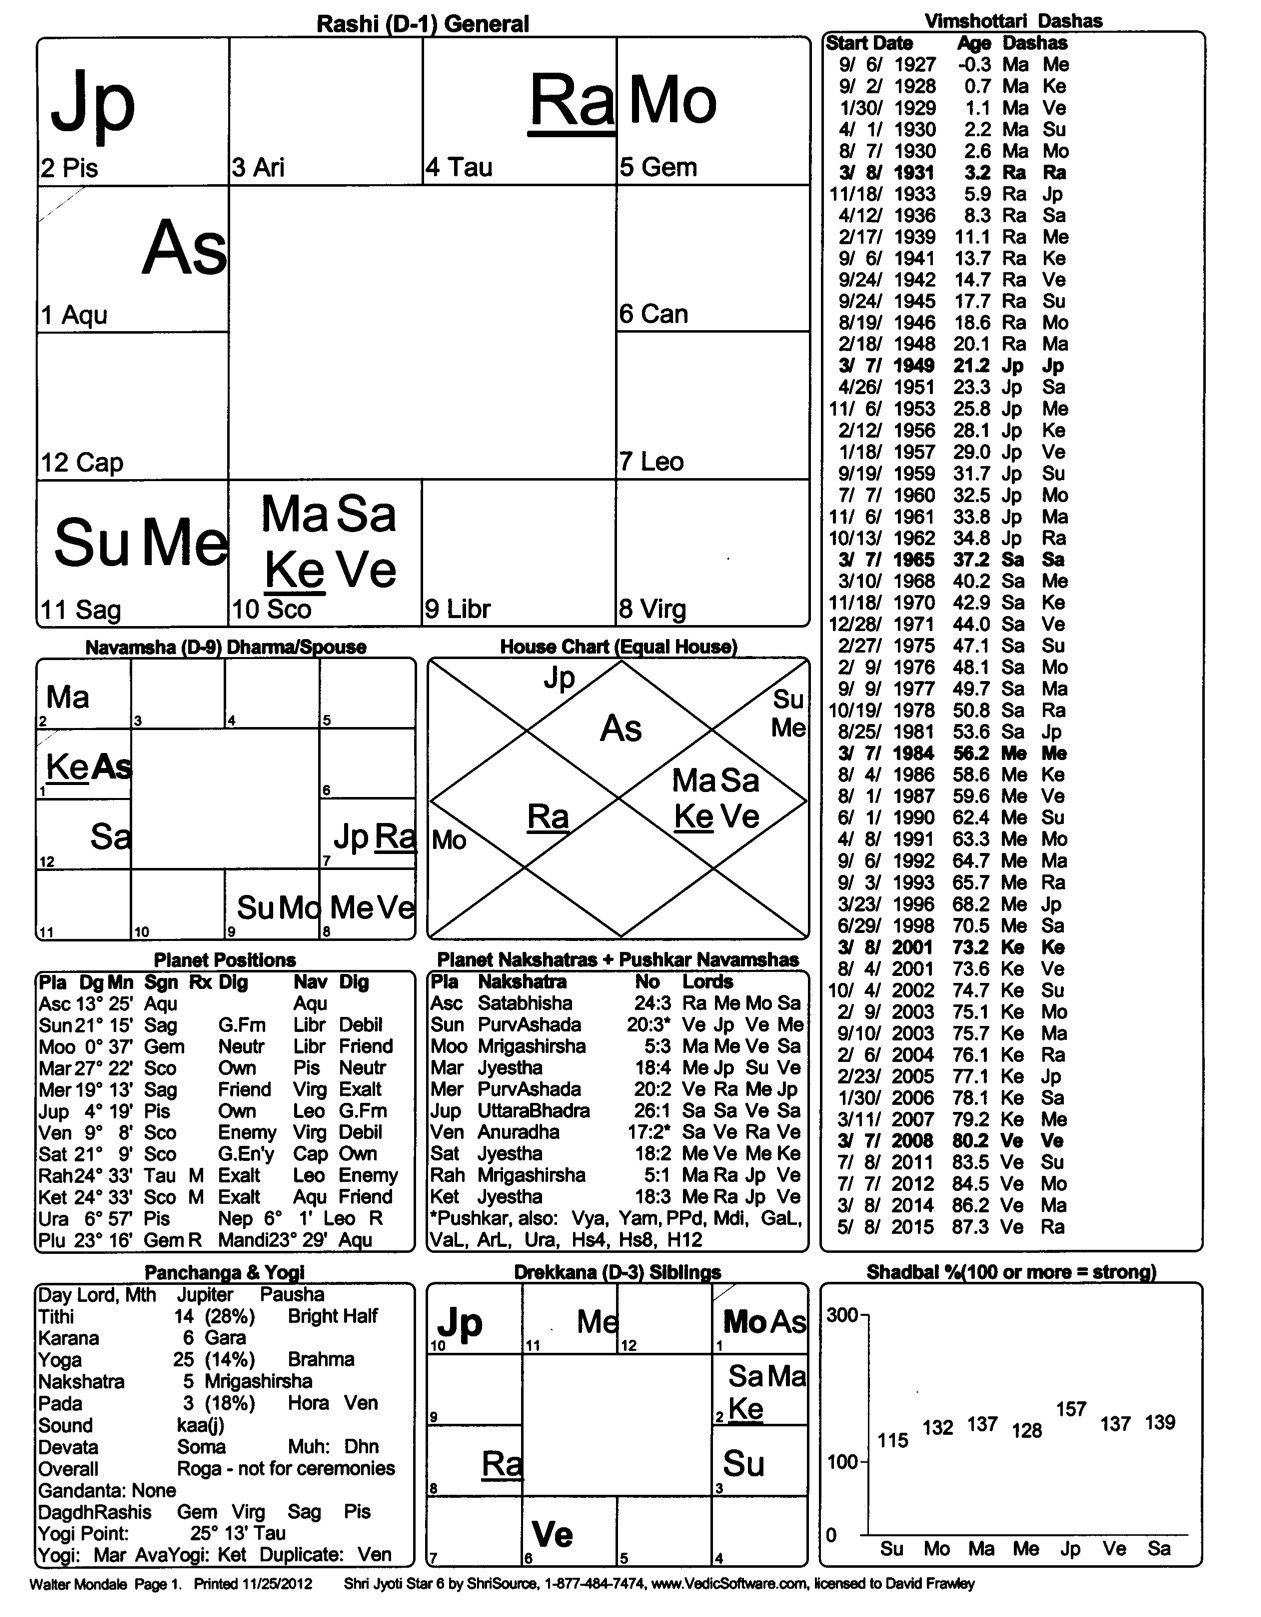
\includegraphics[width=10cm]{pics/Mondale-1.jpg}
\caption{}
\end{figure}

 

The chart has a compassionate Aquarius Ascendant with a good Moon in Gemini in the fifth house approaching full and aspected by its lord Mercury. This makes the person honest, kind, a writer, counselor and advisor. From the Moon Jupiter, the tenth lord is in the tenth house and in a mutual angle with the Ascendant lord providing another type of Raja Yoga. Jupiter here constitutes a Hamsa Yoga (Maha Purusha Yoga of Jupiter) and Gaja Kesari Yoga (being in an angle from the Moon). Good planets and combinations in the second, fifth and eleventh houses provide wealth, as well as excellent writing and speaking abilities.

 

The native had excellent Dashas starting with Jupiter Maha Dasha when he was 21 in 1949 allowing him to rise quickly in life. Saturns Dasha, running from 1965 – 1984 gave him great gains, including the Vice Presidency in Saturn-Moon in 1976, perhaps the highest advisory position in the world. The very strong Saturn-Mars period, combining the Lagna and tenth lord influences, occurred from Sept. 1977 to Oct. 1978.

 

Mercury Dasha commenced in March of 1984 but did not have the power to sustain him. He ran for the Presidency in Mercury-Mercury and lost badly. Mercury as a planet was not connected with the strong Raja in the tenth house. Other factors contributed to his loss. Aquarius Ascendant is generally not strong politically because it tends to lack charisma, with the Ascendant lord also ruling the twelfth house. Another example of Aquarius Ascendant as President is that of Abraham Lincoln, who had a similar compassion and poor charisma but benefited by assuming power in a time of crisis.

 

That Mondales Raja Yoga involves three natural malefics and only one natural benefic would also not strengthen it as much either. In addition the chart is more of a great advisor than a strong leader. The person was probably too spiritual to stoop to the level necessary to win in this age of showmanship. However timing is an important factor in such passing events as elections. Transits and the annual chart would reveal more.

 

Hence merely having Raja Yogas in the chart is not enough if the Dasha scheme is not favorable for their complete unfoldment. If the Dashas of Raja Yoga planets come too early or too late in life the Yogas may not have much of an effect. Almost any chart has some kind of a Raja Yoga. The periods of these planets will be among the natives best but these Yogas may produce only ordinary gains and not counter the effects of an overall weak chart if there is nothing else to support them.

